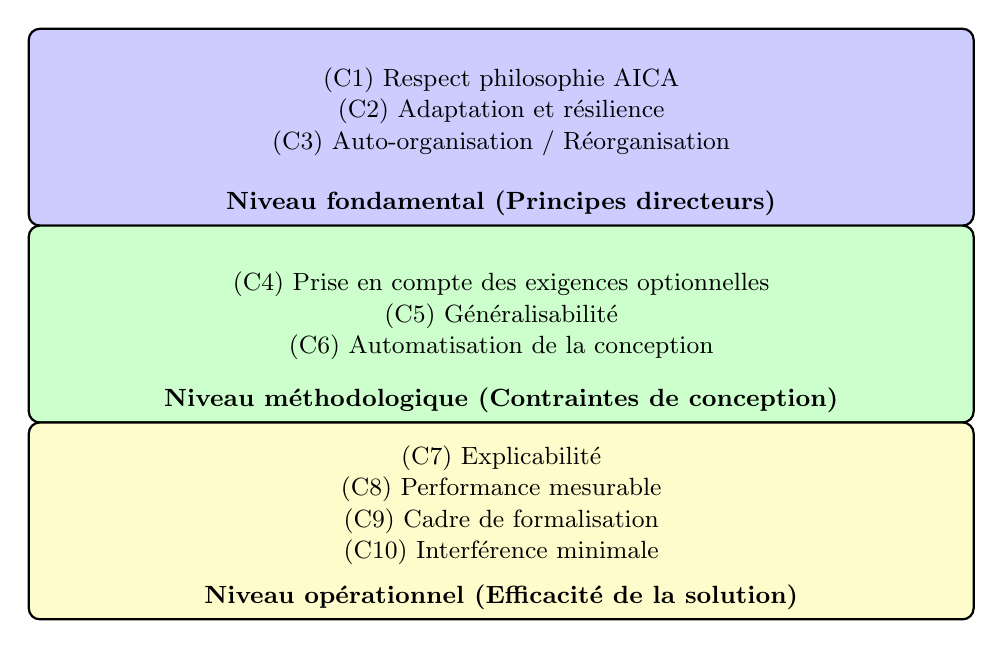
\begin{tikzpicture}[
        levelbox/.style={draw, rounded corners, thick, minimum width=12cm, fill=#1!20},
        itemtext/.style={align=center, font=\small},
        titletext/.style={font=\bfseries\small, yshift=0.3cm},
        node distance=0.4cm
    ]

    % NIVEAU FONDAMENTAL
    \node[levelbox=blue, minimum height=2.5cm] (fundamental) at (0, 5) {};
    \node[titletext, align=center] at (fundamental.south) {Niveau fondamental (Principes directeurs)};
    \node[itemtext] at (0, 5.6) {(C1) Respect philosophie AICA};
    \node[itemtext] at (0, 5.2) {(C2) Adaptation et résilience};
    \node[itemtext] at (0, 4.8) {(C3) Auto-organisation / Réorganisation};

    % NIVEAU MÉTHODOLOGIQUE
    \node[levelbox=green, minimum height=2.5cm] (methodo) at (0, 2.5) {};
    \node[titletext, align=center] at (methodo.south) {Niveau méthodologique (Contraintes de conception)};
    \node[itemtext] at (0, 3.0) {(C4) Prise en compte des exigences optionnelles};
    \node[itemtext] at (0, 2.6) {(C5) Généralisabilité};
    \node[itemtext] at (0, 2.2) {(C6) Automatisation de la conception};

    % NIVEAU OPÉRATIONNEL
    \node[levelbox=yellow, minimum height=2.5cm] (operationnel) at (0, 0) {};
    \node[titletext, align=center] at (operationnel.south) {Niveau opérationnel (Efficacité de la solution)};
    \node[itemtext] at (0, 0.8) {(C7) Explicabilité};
    \node[itemtext] at (0, 0.4) {(C8) Performance mesurable};
    \node[itemtext] at (0, 0) {(C9) Cadre de formalisation};
    \node[itemtext] at (0, -0.4) {(C10) Interférence minimale};

\end{tikzpicture}
